% Created 2024-10-18 vie 16:18
% Intended LaTeX compiler: pdflatex
\documentclass[10pt]{article}
\usepackage[utf8]{inputenc}
\usepackage{lmodern}
\usepackage[T1]{fontenc}
\usepackage[top=1in, bottom=1.in, left=1in, right=1in]{geometry}
\usepackage{graphicx}
\usepackage{longtable}
\usepackage{float}
\usepackage{wrapfig}
\usepackage{rotating}
\usepackage[normalem]{ulem}
\usepackage{amsmath}
\usepackage{textcomp}
\usepackage{marvosym}
\usepackage{wasysym}
\usepackage{amssymb}
\usepackage{amsmath}
\usepackage[theorems, skins]{tcolorbox}
\usepackage[version=3]{mhchem}
\usepackage[numbers,super,sort&compress]{natbib}
\usepackage{natmove}
\usepackage{url}
\usepackage[cache=false]{minted}
\usepackage[strings]{underscore}
\usepackage[linktocpage,pdfstartview=FitH,colorlinks,
linkcolor=blue,anchorcolor=blue,
citecolor=blue,filecolor=blue,menucolor=blue,urlcolor=blue]{hyperref}
\usepackage{attachfile}
\usepackage{setspace}
\usepackage[spanish, ]{babel}
\date{}
\title{Ejercicio de identificación de un modelo ARIMA}
\begin{document}

\maketitle
\section*{Datos}
\label{sec:orgc6fbc2d}

Cargue la serie de datos simulados \href{IdentificaEstosARIMA/f7dcbd-12.gdt}{f7dcbd-12.gdt}

\begin{minted}[frame=lines,fontsize=\scriptsize,linenos=]{r}
open IdentificaEstosARIMA/f7dcbd-12.gdt
\end{minted}
\subsection*{Tareas a realizar}
\label{sec:orgacb41fc}

\begin{enumerate}
\item \hyperref[sec:orgc654ec2]{Realice un primer análisis gráfico: haga
un gráfico de la serie y un gráfico \emph{rango-media}}
\item \hyperref[sec:orge7ea248]{Determine si es necesario transformar logarítmicamente los datos}
\item \hyperref[sec:orgd333deb]{Determine si es necesario tomar una o
más diferencias regulares de la serie}
\item \hyperref[sec:orgc1c2f3e]{Determine si es necesario tomar una
diferencia estacional de la serie}
\item \hyperref[sec:orgc1f5cb2]{Encuentre un modelo ARIMA para la
serie que sea lo más parsimonioso posible, pero cuyos residuos se
puedan considerar \emph{ruido blanco}.}
\end{enumerate}
\section*{Primer análisis gráfico}
\label{sec:orgc654ec2}


\begin{minted}[frame=lines,fontsize=\scriptsize,linenos=]{r}
gnuplot x --time-series --with-lines --output="SerieEnNiveles.png"
rmplot  x --output="rango-media.png"
\end{minted}

\begin{center}
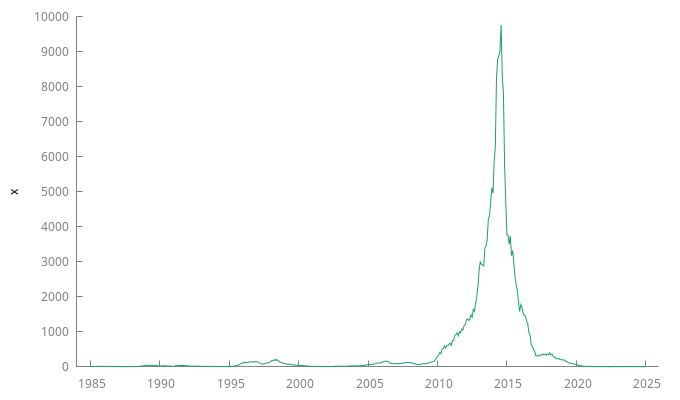
\includegraphics[width=0.5\textwidth]{./EjercicioIdentificacionModeloARIMA/SerieEnNiveles.png}
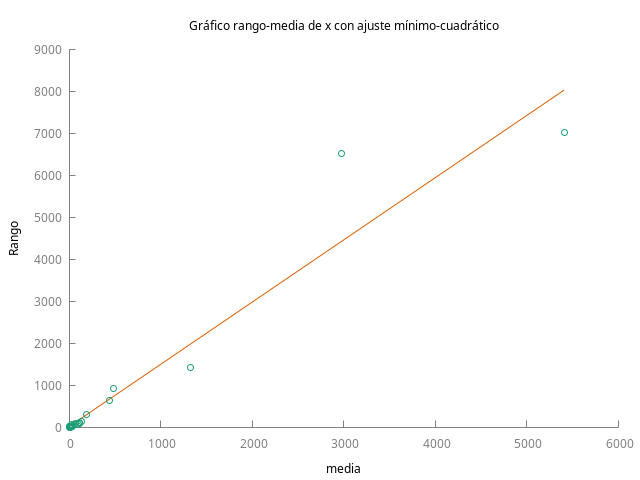
\includegraphics[width=0.4\textwidth]{./EjercicioIdentificacionModeloARIMA/rango-media.png} 
\end{center}
\section*{Estacionariedad en varianza}
\label{sec:orge7ea248}

A la luz de los anteriores gráficos, donde se aprecia que la
variabilidad de los datos aumenta con el nivel de la serie, \textbf{parece
necesaria la transformación logarítmica.}
\subsection*{Transforme logarítmicamente los datos y grafíquelos}
\label{sec:orgc1a5d7d}

\begin{minted}[frame=lines,fontsize=\scriptsize,linenos=]{r}
logs x
gnuplot l_x --time-series --with-lines --output="SerieEnLogs.png"
rmplot  l_x --output="rango-media-enLogs.png"
\end{minted}

\begin{center}
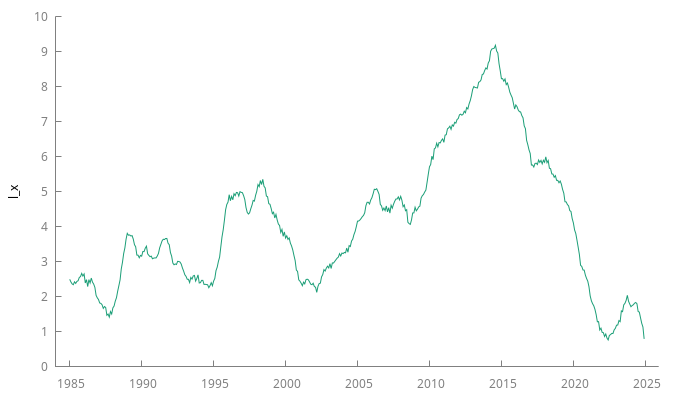
\includegraphics[width=0.5\textwidth]{./EjercicioIdentificacionModeloARIMA/SerieEnLogs.png}
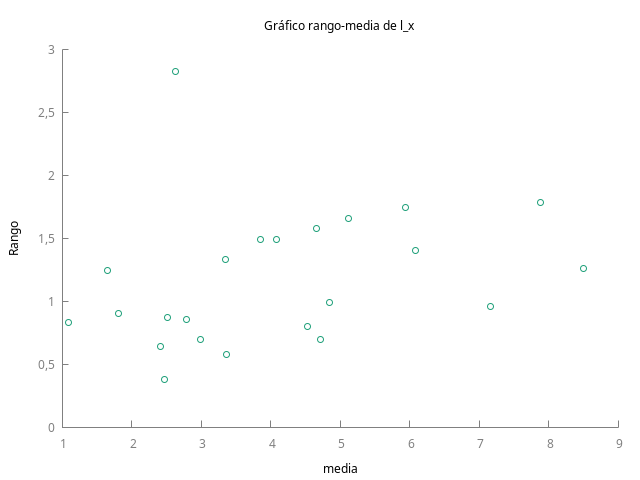
\includegraphics[width=0.4\textwidth]{./EjercicioIdentificacionModeloARIMA/rango-media-enLogs.png} 
\end{center}

La serie en logs ya parece estacionaria en varianza.
\section*{Estacionariedad en media}
\label{sec:orgd333deb}

El gráfico de la serie \texttt{l\_x} parece mostrar una evolución en su nivel
(una tendencia). Por tanto, parece indicado tomar una diferencia
ordinaria.

No obstante, probemos a ajustar un modelo AR(1), probablemente
obtendremos un polinomio autoregresivo con una raíz muy próxima a uno
(o incluso menor que uno en valor absoluto). 

\begin{minted}[frame=lines,fontsize=\scriptsize,linenos=]{r}
AR1 <- arima 1 0 0 ; l_x
\end{minted}


\begin{verbatim}
Evaluaciones de la función: 93
Evaluaciones del gradiente: 24

AR1: ARMA, usando las observaciones 1985:01-2024:12 (T = 480)
Estimado usando AS 197 (MV exacta)
Variable dependiente: l_x
Desviaciones típicas basadas en el Hessiano

             coeficiente   Desv. típica      z      valor p
  ---------------------------------------------------------
  const       2,43628       1,71557         1,420   0,1556 
  phi_1       0,998052      0,00178662    558,6     0,0000  ***

Media de la vble. dep.  4,117853   D.T. de la vble. dep.   1,982703
Media de innovaciones  −0,000257   D.T. innovaciones       0,124169
R-cuadrado              0,996075   R-cuadrado corregido    0,996075
Log-verosimilitud       317,4684   Criterio de Akaike     −628,9367
Criterio de Schwarz    −616,4154   Crit. de Hannan-Quinn  −624,0149

                       Real Imaginaria     Módulo Frecuencia
  -----------------------------------------------------------
  AR
   Raíz  1           1,0020     0,0000     1,0020     0,0000
  -----------------------------------------------------------

AR1 guardado
\end{verbatim}


Tal como se anticipaba, la raíz es casi \texttt{1}. También podemos probar
con los test formales de raíz unitaria
\subsection*{Test ADF}
\label{sec:org9a2ba0c}

\begin{minted}[frame=lines,fontsize=\scriptsize,linenos=]{r}
adf -1 l_x --c --gls --test-down --perron-qu 
\end{minted}

\begin{verbatim}
Contraste aumentado de Dickey-Fuller (GLS) para l_x
contrastar hacia abajo desde 17 retardos, con el criterio AIC modificado, Perron-Qu
tamaño muestral 477
la hipótesis nula de raíz unitaria es: [a = 1]

  contraste con constante 
  incluyendo 2 retardos de (1-L)l_x
  modelo: (1-L)y = b0 + (a-1)*y(-1) + ... + e
  valor estimado de (a - 1): -0,00213547
  estadístico de contraste: tau = -1,19526
  valor p aproximado 0,226
  Coef. de autocorrelación de primer orden de e: -0,013
  diferencias retardadas: F(2, 474) = 156,788 [0,0000]
\end{verbatim}

El  p-valor es elevado, por lo que NO se rechaza la \(H_0\) de que la serie es \(I(1)\)
\subsection*{Test KPSS}
\label{sec:org2792db2}

\begin{minted}[frame=lines,fontsize=\scriptsize,linenos=]{r}
kpss -1 l_x 
\end{minted}

\begin{verbatim}
Contraste KPSS para l_x

T = 480
Parámetro de truncamiento de los retardos = 5
Estadístico de contraste = 1,77747

                      10%      5%      1%
Valores críticos: 0,348   0,462   0,742
Valor p < .01
\end{verbatim}

El  p-valor es menor al 1\%, por lo que se rechaza la \(H_0\) de que la serie es \(I(0)\).

\textbf{Todas las evidencias apuntan a que es necesaria tomar una diferencia ordinaria}
\subsection*{Repetición del análisis con la serie diferenciada}
\label{sec:org4431875}

\begin{minted}[frame=lines,fontsize=\scriptsize,linenos=]{r}
diff l_x
gnuplot d_l_x --time-series --with-lines --output="SerieLogEnDiferencias.png"
\end{minted}

\begin{center}
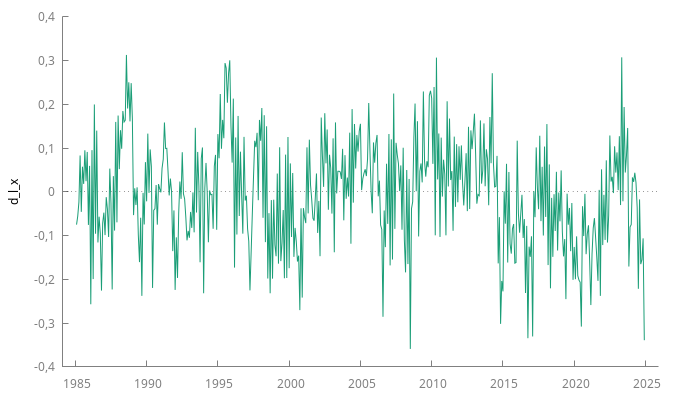
\includegraphics[width=0.5\textwidth]{./EjercicioIdentificacionModeloARIMA/SerieLogEnDiferencias.png}
\end{center}

El gráfico de la serie transformada no muestra tener una clara
tendencia o evolución a largo plazo de su nivel.

Probemos a ajustar un modelo AR a los datos diferenciados

\begin{minted}[frame=lines,fontsize=\scriptsize,linenos=]{r}
ARIMA110 <- arima 1 1 0 ; d_l_x
\end{minted}

\begin{verbatim}
Evaluaciones de la función: 24
Evaluaciones del gradiente: 5

ARIMA110: ARIMA, usando las observaciones 1985:03-2024:12 (T = 478)
Estimado usando AS 197 (MV exacta)
Variable dependiente: (1-L) d_l_x
Desviaciones típicas basadas en el Hessiano

             coeficiente    Desv. típica      z        valor p 
  -------------------------------------------------------------
  const      −0,000361014    0,00262948     −0,1373   0,8908   
  phi_1      −0,755554       0,0299328     −25,24     1,40e-140 ***

Media de la vble. dep. −0,000553   D.T. de la vble. dep.   0,154022
Media de innovaciones   0,000017   D.T. innovaciones       0,100834
R-cuadrado              0,388386   R-cuadrado corregido    0,388386
Log-verosimilitud       417,9912   Criterio de Akaike     −829,9825
Criterio de Schwarz    −817,4736   Crit. de Hannan-Quinn  −825,0647

                       Real Imaginaria     Módulo Frecuencia
  -----------------------------------------------------------
  AR
   Raíz  1          -1,3235     0,0000     1,3235     0,5000
  -----------------------------------------------------------

ARIMA110 guardado
\end{verbatim}

El parámetro \(\phi_1\) está lejos de la unidad (consecuentemente,
también lo está la raíz autorregresiva).

Repitamos también los tests formales
\subsubsection*{Test ADF}
\label{sec:org0894b84}

\begin{minted}[frame=lines,fontsize=\scriptsize,linenos=]{r}
adf -1 d_l_x --c --gls --test-down --perron-qu 
\end{minted}

\begin{verbatim}
Contraste aumentado de Dickey-Fuller (GLS) para d_l_x
contrastar hacia abajo desde 17 retardos, con el criterio AIC modificado, Perron-Qu
tamaño muestral 468
la hipótesis nula de raíz unitaria es: [a = 1]

  contraste con constante 
  incluyendo 10 retardos de (1-L)d_l_x
  modelo: (1-L)y = b0 + (a-1)*y(-1) + ... + e
  valor estimado de (a - 1): -0,145647
  estadístico de contraste: tau = -3,18886
  valor p aproximado 0,001
  Coef. de autocorrelación de primer orden de e: 0,001
  diferencias retardadas: F(10, 457) = 35,578 [0,0000]
\end{verbatim}

El p-valores es muy bajo, por lo que se rechaza la \(H_0\) de que la serie es \(I(1)\)
\subsubsection*{Test KPSS}
\label{sec:org77e7c00}

\begin{minted}[frame=lines,fontsize=\scriptsize,linenos=]{r}
kpss -1 d_l_x 
\end{minted}

\begin{verbatim}
Contraste KPSS para d_l_x

T = 479
Parámetro de truncamiento de los retardos = 5
Estadístico de contraste = 0,542182

                      10%      5%      1%
Valores críticos: 0,348   0,462   0,742
Valor p interpolado 0,039
\end{verbatim}

El p-valor no es muy concluyente: NO se rechaza la \(H_0\) de que la
serie es \(I(0)\) al 1\%, pero sí se rechaza al 5\%. En cualquier caso,
\textbf{las evidencias apuntan mayoritariamente a que NO es necesario tomar
una segunda diferencia ordinaria}
\section*{Diferencias estacionales}
\label{sec:orgc1c2f3e}

Observemos el gráfico de la serie diferenciada y su correlograma.

\begin{minted}[frame=lines,fontsize=\scriptsize,linenos=]{r}
corrgm d_l_x 36 --plot="d_l_x_ACF-PACF.png"
\end{minted}


\begin{center}
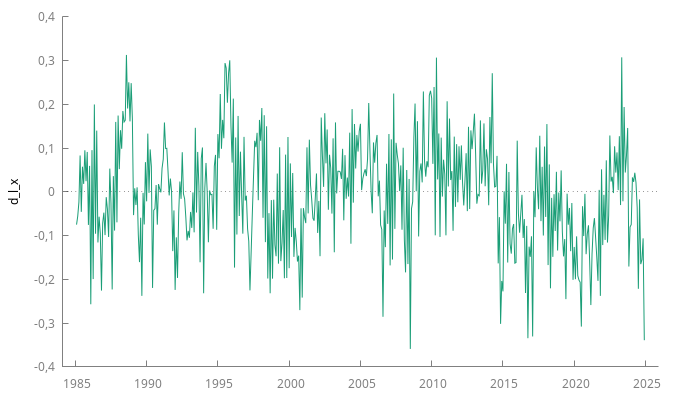
\includegraphics[width=0.5\textwidth]{./EjercicioIdentificacionModeloARIMA/SerieLogEnDiferencias.png}
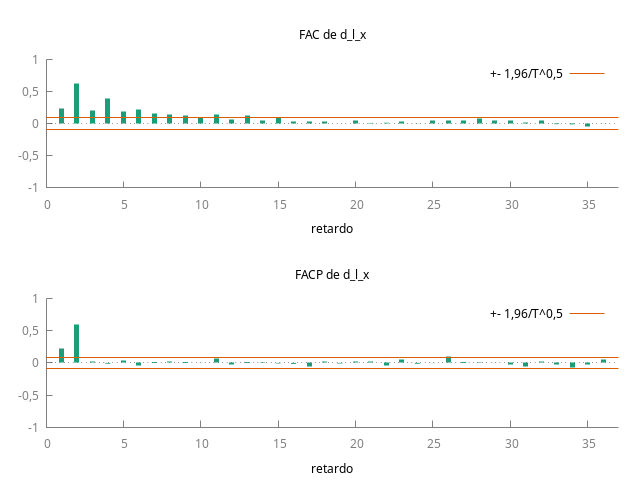
\includegraphics[width=0.5\textwidth]{./EjercicioIdentificacionModeloARIMA/d_l_x_ACF-PACF.png}
\end{center}

Ni en el gráfico de la serie se aprecia ninguna pauta estacional, ni
en la función de autocorrelación simple las correlaciones
correspondientes a los retardos estacionales son significativas (y
deberían ser \textbf{muy prominentes} si fuera necesaria una diferencia
estacional).

Además, si tratamos de ajustar un AR(1) estacional:

\begin{minted}[frame=lines,fontsize=\scriptsize,linenos=]{r}
ARIMA010X100 <- arima 0 1 0 ; 1 0 0 ; l_x  --nc
\end{minted}

\begin{verbatim}
Evaluaciones de la función: 15
Evaluaciones del gradiente: 3

ARIMA010X100:
ARIMA, usando las observaciones 1985:02-2024:12 (T = 479)
Estimado usando AS 197 (MV exacta)
Variable dependiente: (1-L) l_x
Desviaciones típicas basadas en el Hessiano

             coeficiente   Desv. típica     z     valor p
  -------------------------------------------------------
  Phi_1       0,0578266     0,0459270     1,259   0,2080 

Media de la vble. dep. −0,003555   D.T. de la vble. dep.   0,124351
Media de innovaciones  −0,003470   D.T. innovaciones       0,124062
R-cuadrado              0,996083   R-cuadrado corregido    0,996083
Log-verosimilitud       319,9682   Criterio de Akaike     −635,9364
Criterio de Schwarz    −627,5930   Crit. de Hannan-Quinn  −632,6565

                       Real Imaginaria     Módulo Frecuencia
  -----------------------------------------------------------
  AR (estacional)
   Raíz  1          17,2931     0,0000    17,2931     0,0000
  -----------------------------------------------------------

ARIMA010X100 guardado
\end{verbatim}

constatamos que la estimación del parámetro \(\Phi_1\) no es
significativa.

\textbf{Todas las evidencias apuntan a que NO es necesaria tomar ninguna
diferencia estacional}

Recuerde que los test ADF y KPSS no sirven para determinar si es
necesario tomar diferencias estacionales (solo sirven para las
diferencias regulares).
\section*{Búsqueda de un modelo ARIMA}
\label{sec:orgc1f5cb2}

Observando al ACF y la PACF de aprecia que la ACF decae a una tasa
exponencial, y la PACF se trunca tras el segundo retardo, lo cual es
compatible con un AR(2). 

\begin{center}
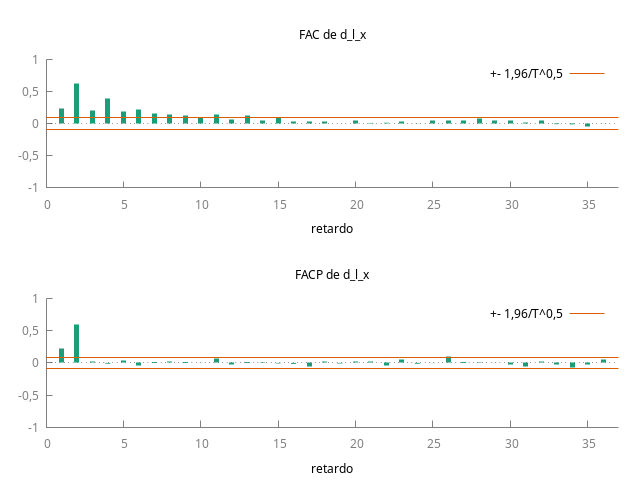
\includegraphics[width=0.5\textwidth]{./EjercicioIdentificacionModeloARIMA/d_l_x_ACF-PACF.png}
\end{center}

Por tanto, parece que la serie en logaritmos sigue un modelo
ARIMA\((2,1,0)\). Veamos si es así:

\begin{minted}[frame=lines,fontsize=\scriptsize,linenos=]{r}
ARIMA210cte <- arima 2 1 0 ; l_x 
\end{minted}

\begin{verbatim}
Evaluaciones de la función: 27
Evaluaciones del gradiente: 6

ARIMA210cte:
ARIMA, usando las observaciones 1985:02-2024:12 (T = 479)
Estimado usando AS 197 (MV exacta)
Variable dependiente: (1-L) l_x
Desviaciones típicas basadas en el Hessiano

             coeficiente   Desv. típica      z      valor p 
  ----------------------------------------------------------
  const      −0,00612415    0,0144972     −0,4224   0,6727  
  phi_1       0,0933620     0,0365714      2,553    0,0107   **
  phi_2       0,604952      0,0365965     16,53     2,22e-61 ***

Media de la vble. dep. −0,003555   D.T. de la vble. dep.   0,124351
Media de innovaciones   0,000230   D.T. innovaciones       0,096517
R-cuadrado              0,997634   R-cuadrado corregido    0,997629
Log-verosimilitud       439,7655   Criterio de Akaike     −871,5310
Criterio de Schwarz    −854,8442   Crit. de Hannan-Quinn  −864,9712

                       Real Imaginaria     Módulo Frecuencia
  -----------------------------------------------------------
  AR
   Raíz  1          -1,3652     0,0000     1,3652     0,5000
   Raíz  2           1,2108     0,0000     1,2108     0,0000
  -----------------------------------------------------------

ARIMA210cte guardado
\end{verbatim}

Los parámetros autorregresivos son significativos y el modulo de las
raíces es claramente mayor que la unidad en ambos casos. No obstante,
la constante no es significativa. 

Reestimemos el modelo sin constante:

\begin{minted}[frame=lines,fontsize=\scriptsize,linenos=]{r}
ARIMA210 <- arima 2 1 0 ; l_x --nc
\end{minted}

\begin{verbatim}
Evaluaciones de la función: 21
Evaluaciones del gradiente: 4

ARIMA210: ARIMA, usando las observaciones 1985:02-2024:12 (T = 479)
Estimado usando AS 197 (MV exacta)
Variable dependiente: (1-L) l_x
Desviaciones típicas basadas en el Hessiano

             coeficiente   Desv. típica     z      valor p 
  ---------------------------------------------------------
  phi_1       0,0936419     0,0365721      2,560   0,0105   **
  phi_2       0,605180      0,0365994     16,54    2,05e-61 ***

Media de la vble. dep. −0,003555   D.T. de la vble. dep.   0,124351
Media de innovaciones  −0,001626   D.T. innovaciones       0,096534
R-cuadrado              0,997634   R-cuadrado corregido    0,997629
Log-verosimilitud       439,6762   Criterio de Akaike     −873,3525
Criterio de Schwarz    −860,8374   Crit. de Hannan-Quinn  −868,4326

                       Real Imaginaria     Módulo Frecuencia
  -----------------------------------------------------------
  AR
   Raíz  1          -1,3652     0,0000     1,3652     0,5000
   Raíz  2           1,2104     0,0000     1,2104     0,0000
  -----------------------------------------------------------

ARIMA210 guardado
\end{verbatim}
\subsection*{Análisis de los residuos}
\label{sec:orge83671a}

Todo parece OK, pero debemos ver el gráfico de los residuos y su
correlograma, así como los estadísticos Q de Ljung-Box para constatar
que podemos asumir que son la realización de un proceso de ruido
blanco. También conviene mirar si tienen distribución gaussiana:


\begin{minted}[frame=lines,fontsize=\scriptsize,linenos=]{r}
series residuos = $uhat
\end{minted}

\begin{minted}[frame=lines,fontsize=\scriptsize,linenos=]{r}
gnuplot residuos --time-series --with-lines --output="Residuos.png"
corrgm residuos 15 --plot="residuosACF-PACF.png"
\end{minted}

\begin{center}
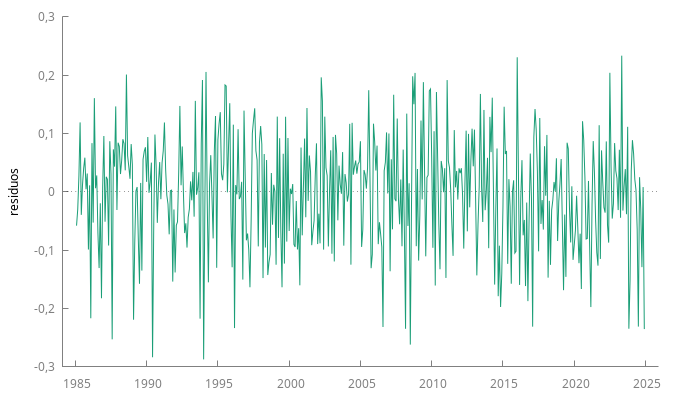
\includegraphics[width=0.5\textwidth]{./EjercicioIdentificacionModeloARIMA/Residuos.png}
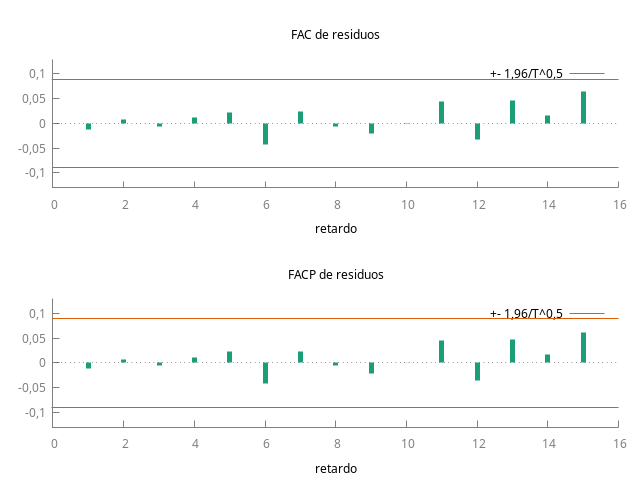
\includegraphics[width=0.5\textwidth]{./EjercicioIdentificacionModeloARIMA/residuosACF-PACF.png}
\end{center}

\begin{minted}[frame=lines,fontsize=\scriptsize,linenos=]{r}
corrgm residuos 15
\end{minted}


\begin{verbatim}
Función de autocorrelación para residuos
***, ** y * indica significatividad a los niveles del 1%, 5% y 10%
utilizando la desviación típica 1/T^0,5

 RETARDO    FAC          FACP         Estad-Q. [valor p]

    1  -0,0115       -0,0115          0,0643  [0,800]
    2   0,0078        0,0077          0,0940  [0,954]
    3  -0,0064       -0,0062          0,1135  [0,990]
    4   0,0112        0,0110          0,1747  [0,996]
    5   0,0218        0,0222          0,4057  [0,995]
    6  -0,0419       -0,0416          1,2590  [0,974]
    7   0,0250        0,0239          1,5640  [0,980]
    8  -0,0067       -0,0054          1,5857  [0,991]
    9  -0,0195       -0,0211          1,7719  [0,995]
   10  -0,0009       -0,0004          1,7723  [0,998]
   11   0,0433        0,0449          2,6954  [0,994]
   12  -0,0331       -0,0353          3,2347  [0,994]
   13   0,0462        0,0479          4,2881  [0,988]
   14   0,0159        0,0178          4,4136  [0,992]
   15   0,0652        0,0623          6,5238  [0,970]
\end{verbatim}

El gráfico de los residuos no presenta ninguna estructura reconocible y ninguna autocorrelación es significativa. 

Más importante aún, \textbf{los correlogramas no muestran ninguna pauta
reconocible, se parecen mucho entre sí y los estadísticos Q muestran
p-valores muy elevados}, por lo que podemos asumir que estos residuos
son ``ruido blanco''.
\medskip

Además, Si en la ventana del modelo estimado pincha en el menú
desplegable \texttt{Gráficos -{}-{}> Espectro con respecto al periodograma
espectral} verá que el espectro teórico del modelo se ajusta
perfectamente al periodograma de la serie.
\medskip

Por tanto, podemos concluir que la serie \texttt{f7dcbd-12.gdt}, una vez
transformada logarítmicamente, sigue un proceso ARIMA\((2,1,0)\) con
media cero. 
\subsection*{Modelo efectivamente simulado}
\label{sec:orge741fd9}

Veamos si ese es el modelo usado en su simulación. Si miramos la línea
\texttt{37} del fichero \href{IdentificaEstosARIMA/000-Etiquetas-12}{000-Etiquetas-12} que se encuentra en el directorio de
donde hemos obtenido los datos encontramos lo siguiente:
\medskip

\begin{center}
\begin{tabular}{l}
\texttt{f7dcbd,	logs,	mu = 2.5,	ar = '(1 - 0.8B)(1 + 0.8B)', ma = '', i = '(1 - B)'}\\
\end{tabular}
\end{center}

\medskip

Efectivamente, requería la transformación logarítmica. La media era
\(2.5\), (es decir la constante simulada no era cero). El polinomio AR
era de grado 2: \(\;\boldsymbol{\phi}=(1 - 0.8\mathsf{B})(1 +
0.8\mathsf{B})=(1+0\mathsf{B}-0.64\mathsf{B}^2)\;\), no tenía
estructura MA y la serie requería una diferencia regular \((1 -
\mathsf{B})\).
\bigskip

Por supuesto que la estimación de los parámetros no coincide
exactamente con los parámetros del modelo simulado, pero la
identificación del modelo ha sido \uline{PERFECTA}.
\bigskip


\textbf{\uline{Ahora escoja al azar nuevas series del \href{https://github.com/mbujosab/EconometriaAplicada-SRC/tree/main/Ejercicios/IdentificaEstosARIMA}{directorio} (dispone de
 centenares de series simuladas con distintos modelos) y practique la
 identificación hasta que adquiera seguridad.}}
\end{document}
